% Created 2022-11-10 Thu 15:17
% Intended LaTeX compiler: pdflatex
\documentclass[presentation,aspectratio=1610]{beamer}
\usepackage[utf8]{inputenc}
\usepackage[T1]{fontenc}
\usepackage{graphicx}
\usepackage{grffile}
\usepackage{longtable}
\usepackage{wrapfig}
\usepackage{rotating}
\usepackage[normalem]{ulem}
\usepackage{amsmath}
\usepackage{textcomp}
\usepackage{amssymb}
\usepackage{capt-of}
\usepackage{hyperref}
\usepackage{khpreamble}
\usepackage{amssymb}
\DeclareMathOperator{\shift}{q}
\DeclareMathOperator{\diff}{p}
\usetheme{default}
\author{Kjartan Halvorsen}
\date{\today}
\title{Discretizing continuous-time controllers}
\hypersetup{
 pdfauthor={Kjartan Halvorsen},
 pdftitle={Discretizing continuous-time controllers},
 pdfkeywords={},
 pdfsubject={},
 pdfcreator={Emacs 26.3 (Org mode 9.4.6)}, 
 pdflang={English}}
\begin{document}

\maketitle


\section{Intro}
\label{sec:orga8428f5}

\section{Discretization}
\label{sec:org7360ea5}
\begin{frame}[label={sec:orgfd75bc5}]{Context}
\begin{itemize}
\item Controller \(F(s)\) obtained from a design in continuous time.
\end{itemize}
\pause
\begin{itemize}
\item Need discrete approxmation in order to implement on a computer
\end{itemize}

\begin{center}
 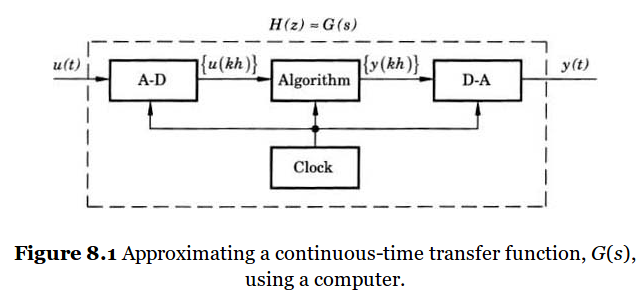
\includegraphics[width=0.7\linewidth]{../../figures/fig8-1.png}\\
 \footnotesize Source: Åström \& Wittenmark 
\end{center}
\end{frame}

\section{Implementation}
\label{sec:orgbb3e09a}
\begin{frame}[label={sec:orgf8415fb}]{Stability for the disk drive arm}
\small 
Case \(\frac{h^2}{J} = 1\). Suggested controller:

\begin{center}
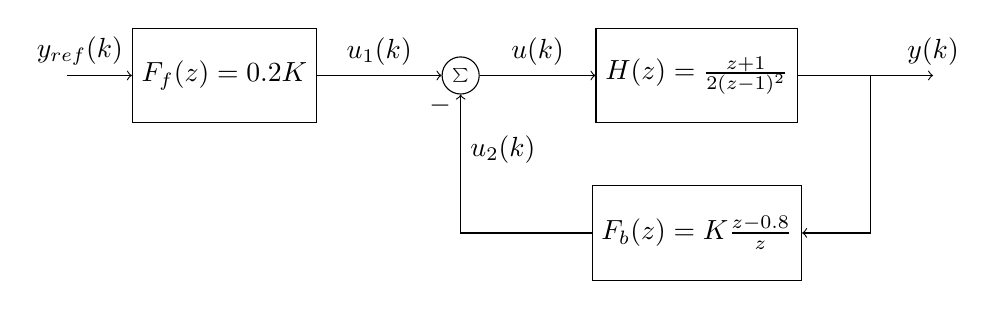
\begin{tikzpicture}
\tikzset{node distance=2cm, 
    block/.style={rectangle, draw, minimum height=12mm, minimum width=14mm},
    sumnode/.style={circle, draw, inner sep=2pt}        
}

  \node[coordinate] (input) {};
  \node[block, right of=input] (TR) {$F_f(z) = 0.2K$};
  \node[sumnode, right of=TR, node distance=30mm] (sum) {\tiny $\sum$};
  \node[block,right of=sum, node distance=30mm] (plant) {$H(z) = \frac{z+1}{2(z-1)^2}$};
  %\node[sumnode, right of=plant, node distance=30mm] (sumdist) {$\sum$};
  %\node[coordinate, above of=sumdist, node distance=15mm] (dist) {};
  %\node[coordinate, right of=sumdist, node distance=15mm] (measure) {};
  \node[coordinate, right of=plant, node distance=30mm] (output) {};
  \node[coordinate, right of=plant, node distance=22mm] (measure) {};
  %\node[sumnode,below of=measure, node distance=25mm] (sumnoise) {$\sum$};
  %\node[coordinate, right of=sumnoise, node distance=15mm] (noise) {};
  \node[block,below of=plant, node distance=20mm] (SR) {$F_b(z)=K\frac{z-0.8}{z}$};
  \draw[->] (input) -- node[above, pos=0.2] {$y_{ref}(k)$} (TR);
  \draw[->] (TR) -- node[above] {$u_1(k)$} (sum);
  \draw[->] (sum) -- node[above] {$u(k)$} (plant);
  \draw[->] (plant) -- node[at end, above] {$y(k)$} (output);
  \draw[->] (measure) |- (SR);
  \draw[->] (SR) -| (sum) node[right, pos=0.8] {$u_2(k)$} node[left, pos=0.96] {$-$};
\end{tikzpicture}
\end{center}
\end{frame}

\section{Preliminaries}
\label{sec:org04f95d9}
\begin{frame}[label={sec:org6fbb414}]{Preliminaries}
\end{frame}


\begin{frame}[label={sec:org9251065}]{Z-transform of a shifted sequence}
\[ x(k) \quad  \overset{\mathcal{Z}}{\longleftrightarrow} \quad X(z)= \sum_{k=0}^{\infty} x(k)z^{-k} \] 
\pause
\[ x(k+1) \quad  \overset{\mathcal{Z}}{\longleftrightarrow} \quad zX(z) - zx(0)\]

\pause
\begin{block}{Proof}
\begin{align*} \ztrf{x(k+1)} &= \sum_{k=0}^{\infty} x(k+1)z^{-k} = \sum_{n=1}^{\infty} x(n)z^{-(n-1)}\\
&=  \sum_{n=1}^{\infty} x(n)z^{-n}z = -zx(0) + z\underbrace{\sum_{n=0}^{\infty} x(n)z^{-n}}_{X(z)}\\
&= zX(z) - zx(0).
\end{align*}
\end{block}
\end{frame}

\begin{frame}[label={sec:orgdbf12f1}]{Discrete-time delay}
\[ x(k-1) \quad  \overset{\mathcal{Z}}{\longleftrightarrow} \quad \frac{1}{z}X(z))\]
\end{frame}


\begin{frame}[label={sec:org45cb9b0}]{Stability for the disk drive arm}
\small 
Case \(\frac{h^2}{J} = 1\). Suggested controller:

\begin{center}
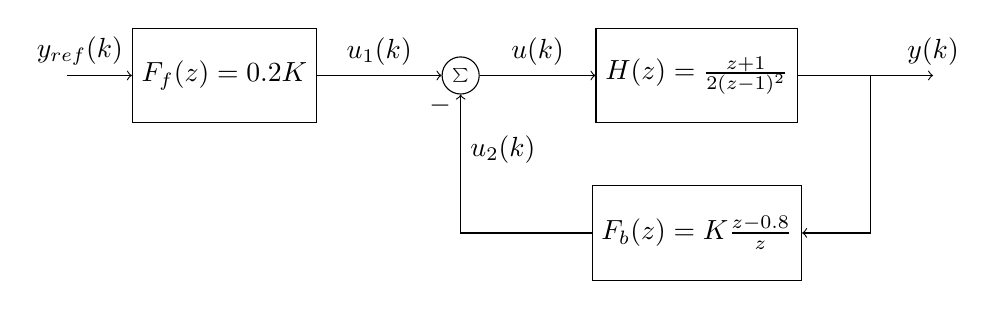
\begin{tikzpicture}
\tikzset{node distance=2cm, 
    block/.style={rectangle, draw, minimum height=12mm, minimum width=14mm},
    sumnode/.style={circle, draw, inner sep=2pt}        
}

  \node[coordinate] (input) {};
  \node[block, right of=input] (TR) {$F_f(z) = 0.2K$};
  \node[sumnode, right of=TR, node distance=30mm] (sum) {\tiny $\sum$};
  \node[block,right of=sum, node distance=30mm] (plant) {$H(z) = \frac{z+1}{2(z-1)^2}$};
  %\node[sumnode, right of=plant, node distance=30mm] (sumdist) {$\sum$};
  %\node[coordinate, above of=sumdist, node distance=15mm] (dist) {};
  %\node[coordinate, right of=sumdist, node distance=15mm] (measure) {};
  \node[coordinate, right of=plant, node distance=30mm] (output) {};
  \node[coordinate, right of=plant, node distance=22mm] (measure) {};
  %\node[sumnode,below of=measure, node distance=25mm] (sumnoise) {$\sum$};
  %\node[coordinate, right of=sumnoise, node distance=15mm] (noise) {};
  \node[block,below of=plant, node distance=20mm] (SR) {$F_b(z)=K\frac{z-0.8}{z}$};
  \draw[->] (input) -- node[above, pos=0.2] {$y_{ref}(k)$} (TR);
  \draw[->] (TR) -- node[above] {$u_1(k)$} (sum);
  \draw[->] (sum) -- node[above] {$u(k)$} (plant);
  \draw[->] (plant) -- node[at end, above] {$y(k)$} (output);
  \draw[->] (measure) |- (SR);
  \draw[->] (SR) -| (sum) node[right, pos=0.8] {$u_2(k)$} node[left, pos=0.96] {$-$};
\end{tikzpicture}
\end{center}
\end{frame}




\section{Warm-up: Differentiation}
\label{sec:org08f1454}

\begin{frame}[label={sec:orgc551c89}]{Differentiation}
\begin{center}
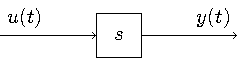
\includegraphics[width=0.5\linewidth]{../../figures/block-simple-derivative}
\end{center}
\end{frame}

\begin{frame}[label={sec:org24ceeec}]{Discrete-time differentiation}
\begin{columns}
\begin{column}{0.4\columnwidth}
\vspace*{5mm}

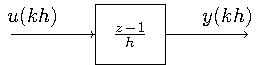
\includegraphics[width=\linewidth]{../../figures/block-simple-discrete-derivative-fwd-z}

\textcolor{white}{Space}

\begin{center}
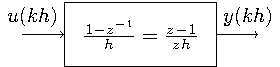
\includegraphics[width=\linewidth]{../../figures/block-simple-discrete-derivative-z}
\end{center}

\alert{Activity} Write as difference equation \[ y(kh) = \] 
\end{column}
\begin{column}{0.6\columnwidth}
\end{column}
\end{columns}
\end{frame}

\section{Implementing the}
\label{sec:org264108b}
\section{Discretization}
\label{sec:orgd2bf2ae}
\begin{frame}[label={sec:orgdab3b62}]{Discretization methods}
\begin{enumerate}
\item Forward difference. Substitute 
\[ s = \frac{z-1}{h} \] in \(F(s)\) to get
\[ F_d(z) = F(s')|_{s'=\frac{z-1}{h}}. \]
\item Backward difference. Substitute 
\[ s = \frac{z-1}{zh} \] in \(F(s)\) to get
\[ F_d(z) = F(s')|_{s'=\frac{z-1}{zh}}. \]
\end{enumerate}
\end{frame}
\begin{frame}[label={sec:org2bf68ab}]{Discretization methods, contd.}
\begin{enumerate}
\setcounter{enumi}{2}
\item Tustin's method (also known as the bilinear transform). Substitute
\[ s = \frac{2}{h}\frac{z-1}{z+1} \] in \(F(s)\) to get
\[ F_d(z) = F(s')|_{s'=\frac{2}{h}\cdot \frac{z-1}{z+1}}. \]
\item Ramp invariance. This is similar to ZoH, which is step-invariant approximation. 
Since a unit ramp has z-transform \(\frac{zh}{(z-1)^2}\) and Laplace-transform \(1/s^2\),  the discretization becomes
\[ F_d(z) = \frac{(z-1)^2}{zh} \ztrf{\laplaceinv{\frac{F(s)}{s^2}}}. \]
\end{enumerate}
\end{frame}

\begin{frame}[label={sec:orgb293404}]{Frequency warping using Tustin's}
\begin{center}
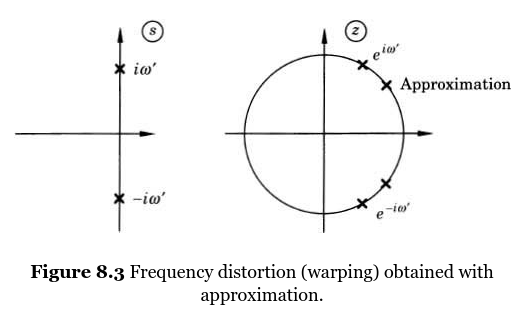
\includegraphics[width=0.6\linewidth]{../../figures/fig8_3.png}
\end{center}
The infinite positive imaginary axis in the s-plane is mapped to the finite-length upper half of the unit circle in the z-plane.
\end{frame}
\begin{frame}[label={sec:org808d8f2}]{Forward difference exercise}
\begin{center}
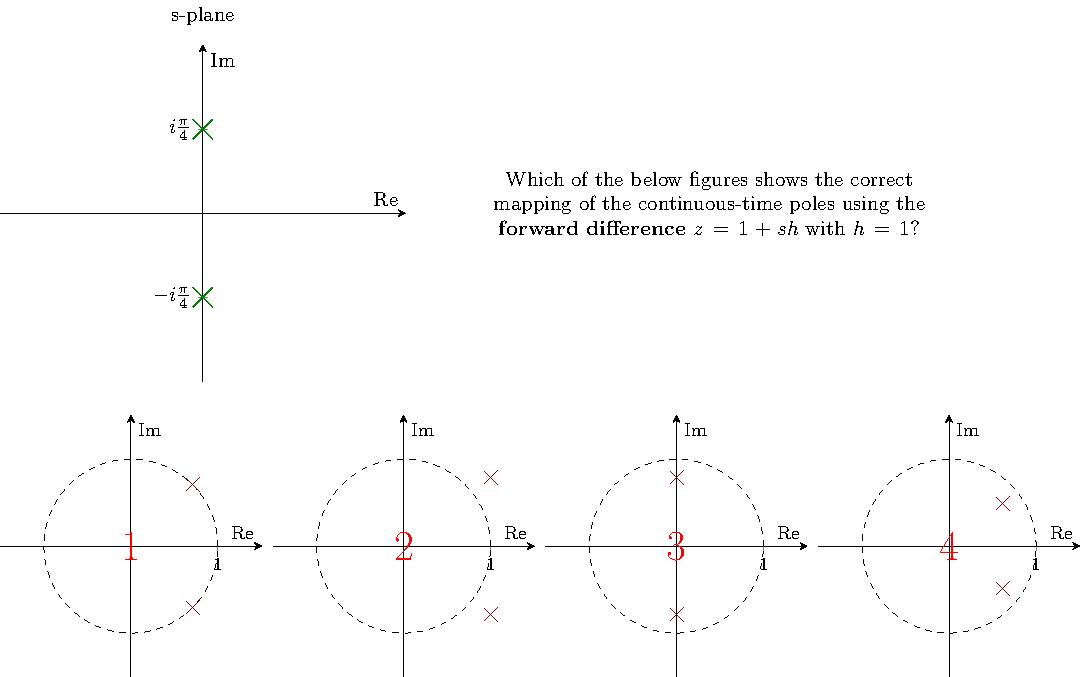
\includegraphics[width=\linewidth]{../../figures/forward-diff-exercise}
\end{center}
\end{frame}

\begin{frame}[label={sec:org87e101f}]{Backward difference exercise}
\begin{center}
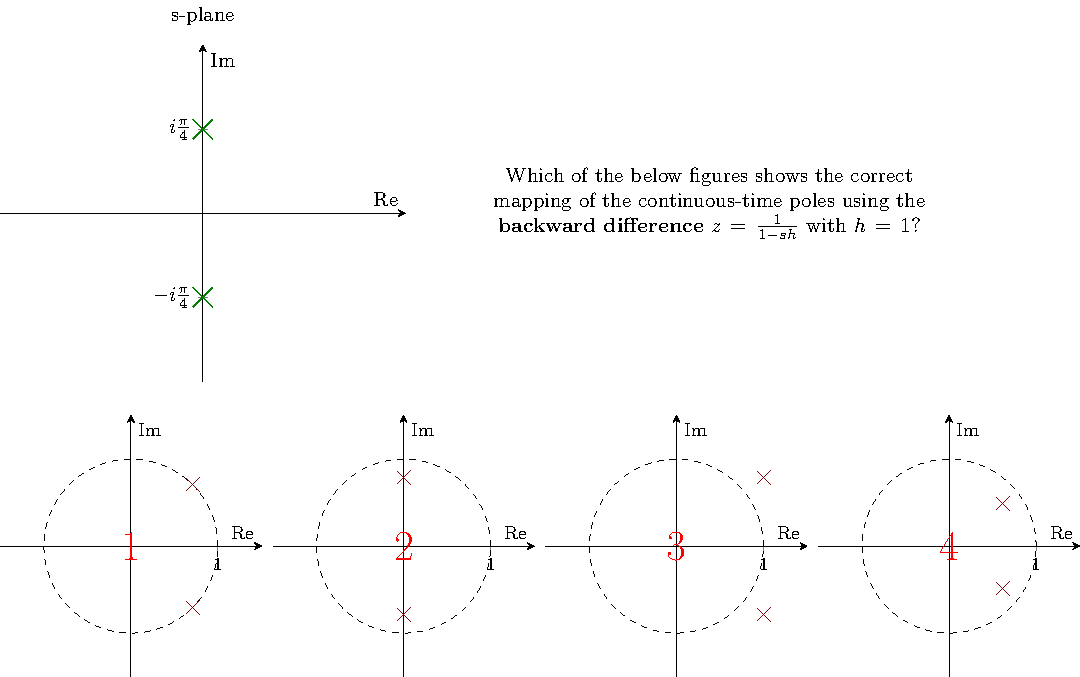
\includegraphics[width=\linewidth]{../../figures/backward-diff-exercise}
\end{center}
\end{frame}
\end{document}